\chapter{Serial Powering}
L'alimentazione seriale dei moduli è una tra i candidati come sistema di distribuzione dell'alimentazione in grado di rispettare i requisiti per un rivelatore a pixel di fase due. 
I chip utilizzati saranno fabbricati in tecnologia CMOS a 65 nm e richiederanno livelli di corrente elevati, fino anche a 2A, al fine di funzionare correttamente nonostante l'alto numero di pixel (canali da leggere) e l'alto rate di eventi.
Inoltre gli alti livelli di radiazione e del campo magnetico insieme al bisogno di minimizzare il più possibile  l'interazione delle particelle con spessori morti scoraggiano l'utilizzo di convertitori DC-DC all'interno del volume del tracciatore. Una soluzione potrebbe essere l'utilizzo di un sistema di alimentazione seriale. 

\section{Caratteristiche dell'alimentazione seriale}
In un sistema di alimentazione seriale il generatore alimenta una catena di moduli, mentre nella classica alimentazione in parallelo la tensione di alimentazione è comune a tutti i moduli ed in ciascuno scorre una corrente diversa.
Questo per sottolineare il fatto che nel caso di alimentazione seriale la corrente è riutilizzata n-volte riducendo così le perdite di potenza nei cavi. 
Trascurando le inefficienze date dal circuito di SLDO possiamo calcolare il rapporto tra la potenza assorbita da n moduli in parallelo con quella di n moduli in serie:
\begin{equation}
W_{parallelo} = n \cdot I \cdot V + (I\cdot n)^2 \cdot R
\end{equation}
\begin{equation}
W_{serie} = n \cdot I \cdot V + I^2 \cdot R
\end{equation}
\begin{equation}
\frac{W_{parallelo}}{W_{serie}} = \frac{1+ \dfrac{nRI}{V}}{1+\dfrac{RI}{Vn}}
\end{equation}
dove R è la resistenza dei cavi, I è la corrente di alimentazione per il singolo modulo e V è la caduta di tensione su ciascun modulo. 
Il punto chiave per una alimentazione seriale è il fatto che la corrente che viene fatta scorrere nella catena sia maggiore o uguale a quella necessaria per alimentare l'elemento della catena con il più alto consumo in termini di potenza e corrente.
Anche nel caso più semplice in cui tutti gli elementi siano uguali rimane il problema, in quanto il comportamento dinamico degli elementi rende necessarie delle ottimizzazioni. 
In qualsiasi momento l'alimentazione deve essere in grado di erogare abbastanza corrente per far fronte ai picchi di assorbimento dei singoli elementi della catena. 
Dal momento che queste variazioni sono molto veloci l'alimentatore, causa la distanza dall'esperimento, i. e. i cavi che trasportano l'alimentazione introducono un ritardo (proporzionale alla lunghezza degli stessi),
non può essere in grado di compensarle in modo rapido, questo è un punto critico che richiede un attento studio. 
Una possibile soluzione consiste nell'implementazione di uno shunt regulator all'interno del chip che converta la corrente in una tensione stabile. 
Nel fare questo è necessario che le fluttuazioni di carico del chip non siano visibili esternamente. 
Lo shunt regulator ha dunque il compito di mantenere costante la corrente totale indipendentemente dal consumo istantaneo del chip.

\section{SLDO}
L'idea più semplice per ottenere un'alimentazione seriale è quella di porre singoli elementi in serie dotati di regulator, questa configurazione ha però una criticità molto importante: il fallimento di un singolo elemento rende inutilizzabile l'intera catena. 
Inoltre in questo modo le fluttuazioni di tensione dei vari elementi influiscono significativamente  sulla tensione generata localmente, per questo motivo è stato progettato uno SLDO (shunt low drop out) voltage regulator.
....
%lo schema consiste in due loop di controllo accoppiati, il primo fa si che il transistor M4 faccia passare tutta la corrente che non è consumata dal carico attivo. Mentre un voltage regulator (A1+M1) assicura che il carico attivo (nel nostro caso RD53A) sia alimentato con una tensione costante, indipendentemente dalla corrente consumata e indipendentemente dalla correte che viene immessa nella catena seriale.
% 
Caratteristica importante dello ShuntLDO è che esternamente è visto come una resistenza efficace $R_{eff}$, in serie ad un offset di tensione $V_{offset}$, mentre il carico attivo, nel nostro caso il chip, non è visibile e dunque non lo sono nemmeno le sue le sue variazioni. 
Questa comportamento resistivo permette l'utilizzo di più SLDO in parallelo tra cui la corrente si suddivide in modo ben preciso, definito dalla resistenza effettiva di ciascun SLDO. Il valore resistivo può essere configurato con una resistenza esterna, consentendo così di definire in che modo la corrente si spartisce nel parallelo di più elementi, ad esempio nel chipRD53A, che verrà trattato nei capitoli seguenti, ci sono due regioni alimentate separatamente da due ShuntLDO, una zona analogica ed una digitale. Esternamente sarà dunque visibile il parallelo tra i due SLDO. Come si può vedere in figura \ref{VVC} I valori di $R_{eff}$ e $V_{offset}$ sono scelti andando a considerare i due punti di lavoro estremi. La tensione minima necessaria al regolatore (all'incirca $1.4V$) deve essere raggiunta con la minima corrente di lavoro, che è data dai consumi del chip. Naturalmente per garantire un corretto funzionamento è necessario fornire un certo margine di corrente in eccesso, vedi figura \ref{SLDOprinciple}. 
\begin{figure}
\centering
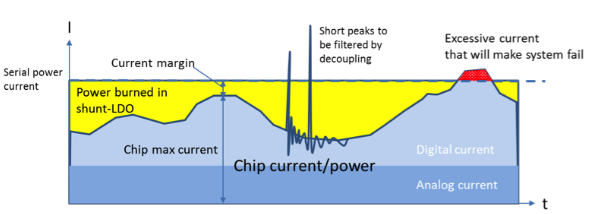
\includegraphics[scale=.5]{Immagini/ShuntRegulatorPrinciple}
\caption{La corrente fornita allo SLDO è costante nel tempo, mentre quella utilizzata dal chip varia. L'aspetto che è importante sottolineare è la necessità di avere una corrente seriale che sia sempre maggiore del massimo carico in corrente.}
\label{SLDOprinciple}
\end{figure}
L'altro estremo nel grafico corrente-tensione è il punto che ha la massima tensione con la massima corrente. Prendendo per buono che non sarà mai utilizzata una corrente maggiore del massimo per alimentare il dispositivo, si ha la sicurezza che nemmeno la tensione massima sarà raggiunta. 
Il consumo in potenza sarà $P=I_{in}^2R_{eff}+I_{in}V_{offset}$, una $R_{eff}$ minore consente di avere minor aumento di potenza all'aumentare della corrente. %e dunque per un corretto funzionamento del chip è possibile utilizzare correnti minori, ovvero lasciando meno margine per le fluttuazioni, proprio perchè con $r_{eff}$ minore le fluttuazioni di corrente
 Dunque al fine di ridurre il consumo di potenza, la resistenza effettiva dello SLDO può avere un offset modificabile. (Low-power mode configuration, che cosa posso dire...).

\begin{figure}
\centering
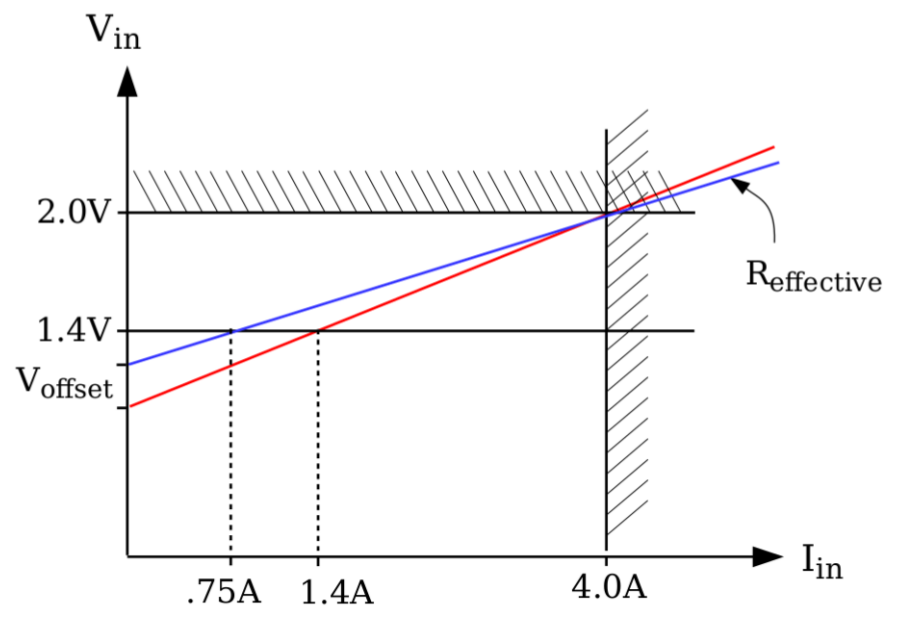
\includegraphics[scale=.3]{Immagini/VoltageVsCurrent}
\caption{Andamento tensione vs corrente del comportamento del chip. Le zone tratteggiate sono oltre i valori operativi massimi (4.0 A per la corrente e 2.0 V per la tensione). La linea orizzontale a 1.4 V è la tensione minima di lavoro. La pendenza è la resistenza efficace, combinazioni differeni di resistenze e offset consentono di spostare il punto di lavoro.}
\label{VVC}
\end{figure}

In un sistema di alimentazione seriale molti chip sono collegati in parallelo all'interno di ciascun modulo, ogni modulo è collegato in serie agli altri, vedi figura \ref{MCM}. 
Come esempio prendiamo la situazione in cui si ha un serie di 8 moduli con 4 chip ciascuno, assumiamo che $V_{offset}=0.8V$ e $R_{eff}=0.3 \Omega$ per ciascun chip\footnote{$R_{eff}$ del singolo SLDO è circa $0.600 \Omega$, nel chip sono presenti due SLDO in parallelo uno per l'alimentazione della parte digitale ed uno per quella analogica. La $R_{eff}$ con cui viene visto il chip è dunque la metà, $0.300\Omega$.}. 
Con una corrente di $I_{in}=2.0 A$ per chip\footnote{Che vale a dire 1A per ciascuno dei due SLDO presenti nel chip.} ($I=8.0 A$ per modulo) si avrà un $V_{modulo}=1.4 V$, per avere margine si pone la corrente seriale $20 \%$ maggiore, $I=9.6A$. 
In questa situazione $V_{modulo}=1.52V$, la caduta di tensione su tutta la catena formata da 8 moduli è $12.16V$, inoltre c'è una resistenza dovuta ai cavi, assumiamo $2 \Omega$. 
La tensione di uscita del generatore è dunque $V=I \cdot 2 \Omega +12.6V=31.8V$\footnote{Circa il $60 \%$ della potenza è dissipato sui cavi, questa fatto potrebbe sembrare un pessimo traguardo, in realtà è un miglioramento rispetto alla situazione attuale.}. 
Il generatore sarà limitato in corrente , mentre il limite per la tensione sarà posto leggermente maggiore ad esempio 34 V. 
In questo modo la potenza che il generatore può erogare è maggiore di quella necessaria per la catena, questo è utile nel caso in cui alcuni chip smettano di funzionare. 
La potenza massima erogabile è dunque $34V \cdot 9.6 A = 326.4 W$, sottraendo la potenza dissipatasui cavi e dividendo per il numero di moduli si ottiene una potenza per modulo di $17.76 W$, a fronte  di una potenza arrorbita nelle normali condizioni di lavoro di $W = 4 \cdot W_{chip} = I \cdot V_{modulo} = 14.6 W$.

\begin{figure}
\centering
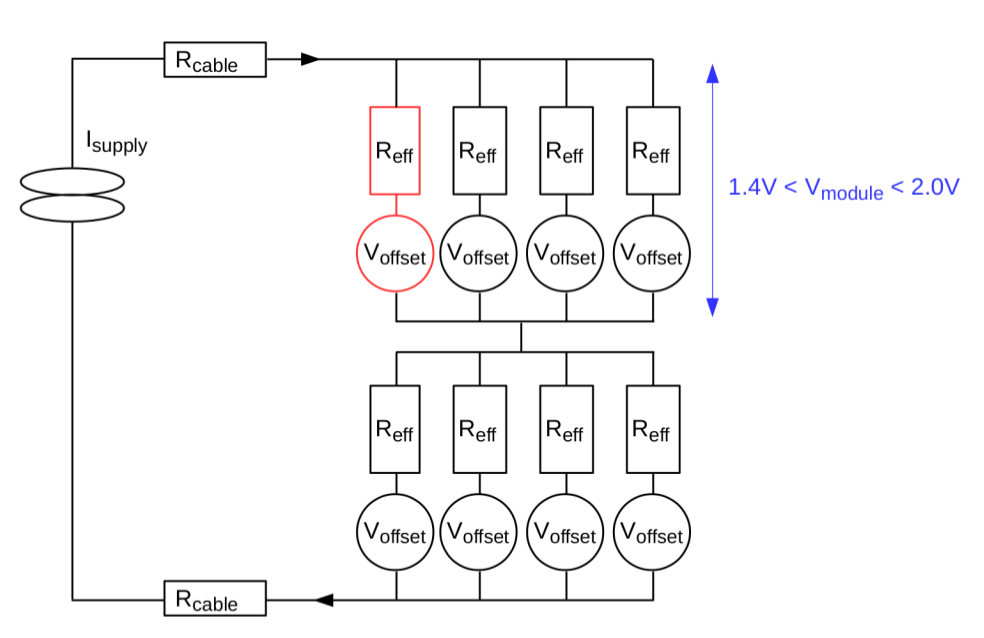
\includegraphics[scale=.3]{Immagini/MultiChipModules}
\caption{Schema di una catena seriale con moduli, ognuno formato da 4 chip. Il chip in rosso si riferisce all'ipotesi di un failure.}
\label{MCM}
\end{figure}

A questo punto possiamo chiederci cosa succeda nel caso in cui un chip in uno dei moduli sia fuori uso\footnote{Dal momento che nel chip ci sono due SLDO lo scenario più probabile è che solo uno dei due sia danneggiato.} 
Dato che l'alimentazione è in corrente ciascuno dei tre chip rimanenti dovrà assorbire un terzo di corrente in più, dunque la corrente per ciascun chip sarà $ I = 9.6 / 3 = 3.2 A$. 
Perciò $V_{modulo} = 3.2 A \cdot 0.3 \Omega + 0.8 V = 1.76 V$, la potenza dissipata su questo modulo sarà $W = 3 \cdot W_{chip} = 3 \cdot I \cdot V_{modulo} = 16.9 W$, un incremento di $2 W$ sul singolo modulo, che corrisponde al $13 \%$. Per la catena di 8 moduli l'incremento è appena di $1.7\%$. 
Questo causerà anche un lieve aumento della tensione erogata dal generatore, che però rimarrà sotto ai 34 V.\footnote{Come visto alla tensione massima di  34 V il generatore riesce a distribuire una potenza di $17.76$ W per ciascun modulo.} 


Lo studio dell'alimentazione seriale parte dunque dalla caratterizzazione dello SLDO. Componente che sarà poi utilizzato all'interno del chip RD53A per la generazione delle tensioni di alimentazione della parte analogica e digitale. .......continuare discorso....


\section{Evoluzione design SLDO}
Il design dello shunt ha subito nel tempo modifiche e migliorie, fino ad arrivare all'attuale versione in tecnologia CMOS a 65 nm capace di lavorare con una corrente massima di 2A.

\begin{figure}
\centering
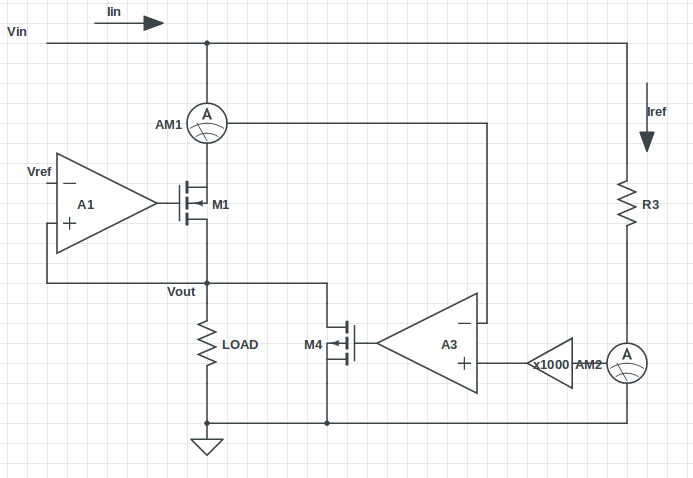
\includegraphics[scale=.4]{Immagini/SLDOprova}
\caption{Schema di principio dello SLDO.}
\label{SLDOprova}
\end{figure}

Partiamo da uno schema estremamente semplificato, figura \ref{SLDOprova}, lo shunt è alimentato in corrente $I_in$, una frazione di questa corrente scorrerà nel ramo con R3, la indichiamo con $I_{ref}$, questa sarà la corrente di riferimento all'interno dello shunt. 
Infatti la parte di Voltage regulator è svolta da A1 tiene la tensione sul carico uguale ad una di riferimento, per ora trascuriamo come sia generata, andando ad aprire o chiudere il gate del mosfet M1 e dunque facendo scorrere più o meno corrente. 
Questo di per se causerebbe un aumento di $I_ref$ e conseguentemente di $V_in$ con un rapporto dato da R3. Nello schema è però presente un ramo in parallelo al carico, in cui la corrente che scorre è regolata da M4+A3, A3 è la parte attiva dello shunt, che fa sì che la corrente nel ramo con M1 sia 1000 volte quella che scorre in R3 andando a regolare $I_{shunt}$ modificando la tensione di gate del mosfet M4. 
La corrente che scorre in M1 è dunque tenuta costante anche quando si hanno variazioni dinamiche del carico.

\begin{figure}
\centering
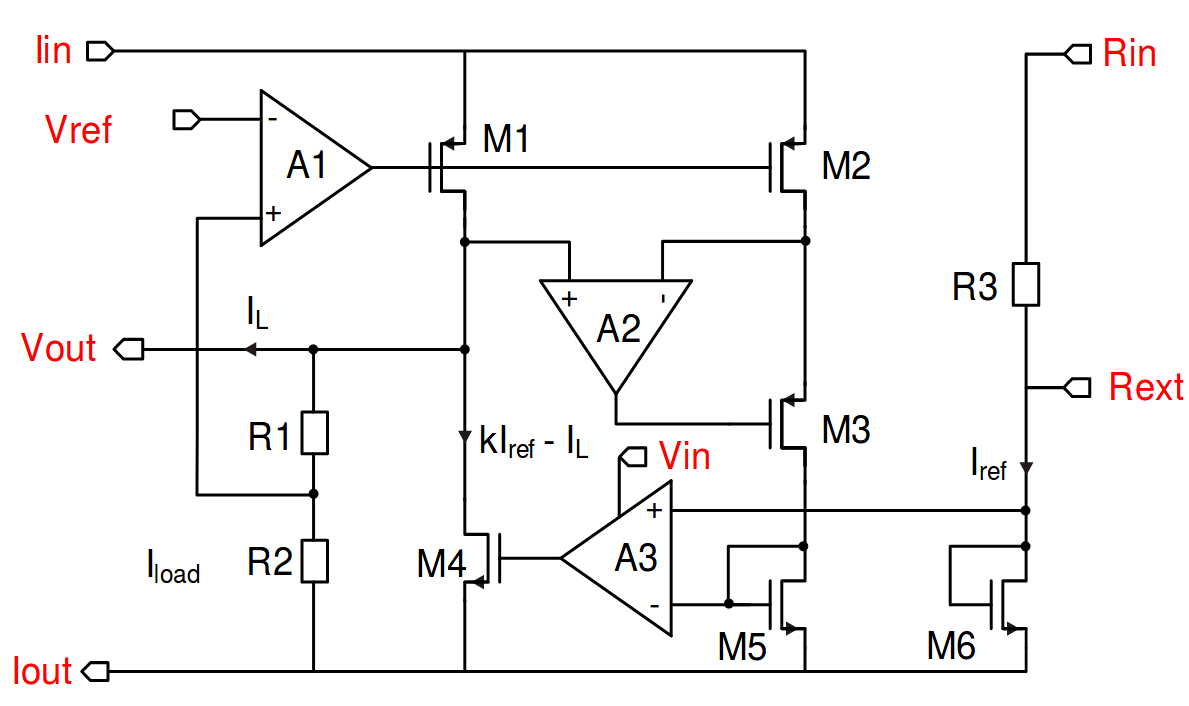
\includegraphics[scale=.3]{Immagini/SLDO5A}
\caption{Circuito semplificato dello SLDO 0.5 A.}
\label{SLDO5A}
\end{figure}

Questo primo schema permette una comprensione generale del funzionamento dell'oggetto il cui schema semplificato nella versione da $0.5 A$ è riportato in figura (figura). Rispetto a quanto visto fino ad ora si hanno alcune differenze, benché l'idea generale di funzionamento rimanga la stessa. 
In questo schema il carico sta tra i pin $V_{out}$ e $I_{out}$ in parallelo al partitore R1+R2 (R1 e R2 sono resistenze uguali), la tensione di riferimento $V_ref$ è confrontata con la tensione su R2 che è la metà di $V_{out}$. A3 fa un confronto tra le correnti che scorrono nel ramo di R3 $I_{ref}$ e in quello di M2 e di conseguenza regola M4. La coppia di mosfet M1-M2 è in configurazione current-mirror e il rapporto k tra le due correnti è uguale a 1000 (dato dalle caratteristiche geometriche dei due mosfet). 
Quindi la corrente che scorre in M1 è 1000 volte $I_{ref}$. Questo comportamento ci dice che esternamente lo SLDO è visto come un carico resistivo circa uguale a $\frac{R3}{k}$. A2+M3 ha lo scopo di migliorare la precisione di k, tenendo uguale la tensione. Il valore di R3 per quanto detto è una importante caratteristica, e la sua scelta determina la tensione nel punto di lavoro del grafico IV per una data corrente. 
Per funzionare è necessaria una tensione in ingresso minima di circa $1.4V$, dunque valori di resistenza maggiori consentiranno di operare con correnti minori(in quanto perché lo SLDO funzioni è necessaria una tensione minima) con il vantaggio di consumare minor potenza (in quanto la corrente in ingresso è fissata e quella non utilizzata viene dissipata sullo shunt che diventa un punto molto caldo), ma con lo svantaggio di aver minor spazio per eventuali fluttuazioni del carico. 
Analogamente resistenze minori avranno l'effetto contrario, tensioni minori a correnti maggiori.
Sempre nello schematico è indicato con $R_{ext}$ il punto in cui è possibile collegare una resistenza esterna in sostituzione ad R3, che è quella presente di default all'interno dello SLDO.
\begin{figure}
\centering
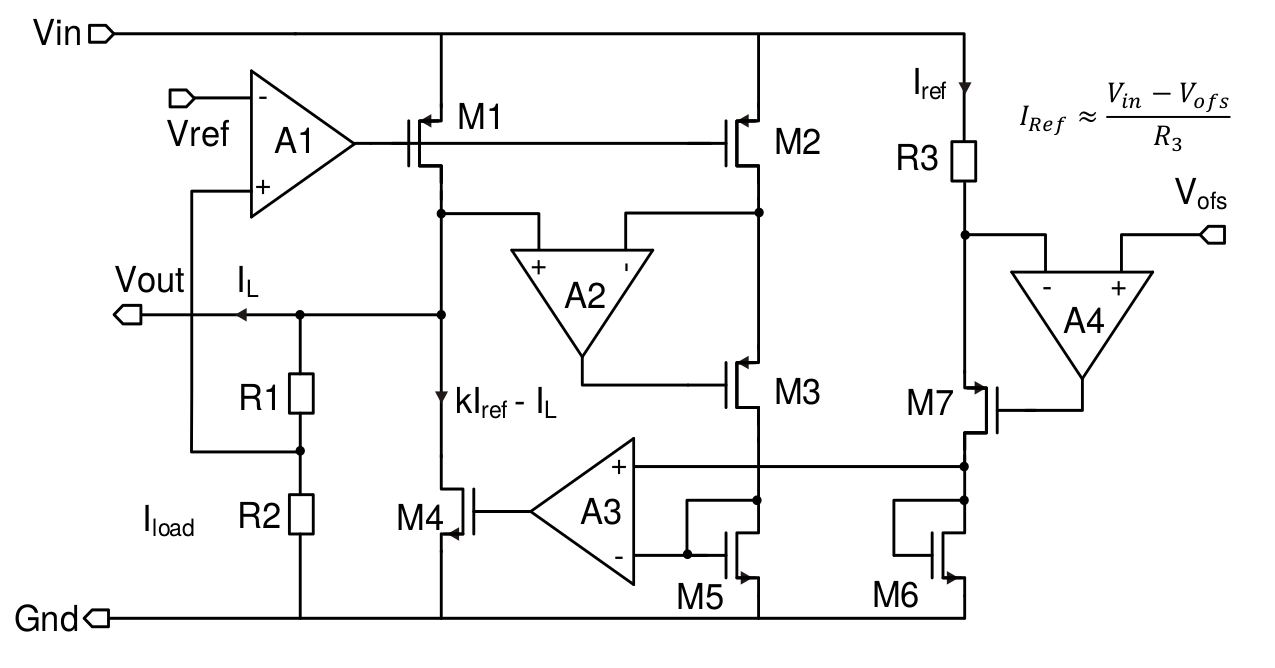
\includegraphics[scale=.3]{Immagini/SLDO2A}
\caption{Circuito semplificato dello SLDO 2A.}
\label{SLDO2A}
\end{figure}
Nel prototipo a $2A$, rispetto alla versione a $0.5A$, è presente il mosfet M7 sul ramo di R3, il cui gate è controllato da A4 (vedi figura \ref{SLDO2A}). Questo ulteriore stadio inserisce un offset di tensione al comportamento resistivo dello SLDO.

\subsection{PCB}
Questa prima parte di studio del comportamento dello SLDO è stato eseguita utilizzando PCB di test nella cui parte centrale lo ShuntLDO è stato collocato e connesso con wire-bond. La PCB riportata nelle immagini è quella relativa al prototipo di ShuntLDO da 2A, figura \ref{PCBTestSLDO}. 
Sulla PCB sono presenti connettori molex per l'alimentazione, jumper di configurazione, pin per misurare varie tensioni etc. Per semplicità e chiarezza espositiva verranno introdotti solo gli elementi principali.

\begin{figure}
\centering
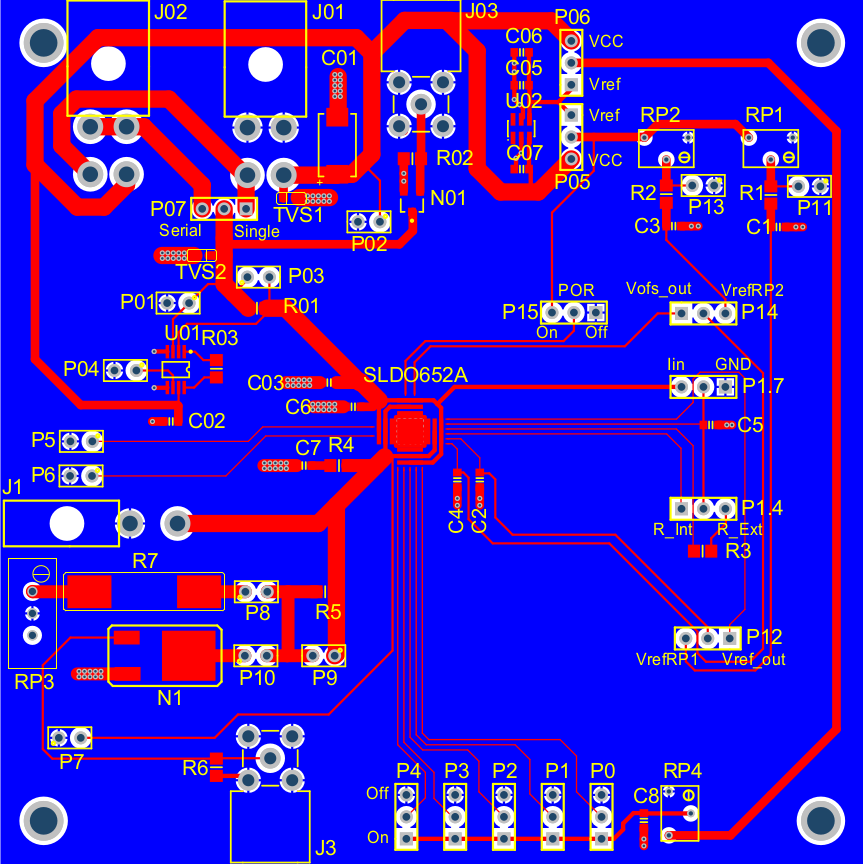
\includegraphics[scale=.3]{Immagini/chipcard}
\caption{PCB di Test per lo SLDO 2A.}
\label{PCBTestSLDO}
\end{figure}

Aggiungere immagini reali.....

L'alimentazione è fornita tramite il molex J01 la linea 1 fornisce la tensione Vcc utilizzata dal bandgap U02 per la generazione del Vref.

\section{Caratterizzazione ShuntLDO da 0.5A}
Le prime misure sono state fatte sul prototipo di SLDO da 0.5A prima del passaggio alla versione 2A. La PCB utilizzata è perciò leggermente differente da quella descritta nella sezione precedentte, sebbene le funzionalità principali rimangano le stesse. Unica differenza sostanziale è la possibilità di inserire un offset regolabile al $V_{out}$, cosa che è invece possibile con la PCB dello SLDO da 2A.
Il primo studio affrontato è stato la caratterizzazione dello SLDO, alimentando in corrente il circuito, e misurando le tensioni in vari punti di interesse. Le prime misure eseguite sono state dunque le IV andando a misurare la tensione in ingresso $V_{in}$, di uscita $V_{out}$ e quella di riferimento $V_{ref}$ in funzione della corrente in ingresso.
\begin{figure}
\centering
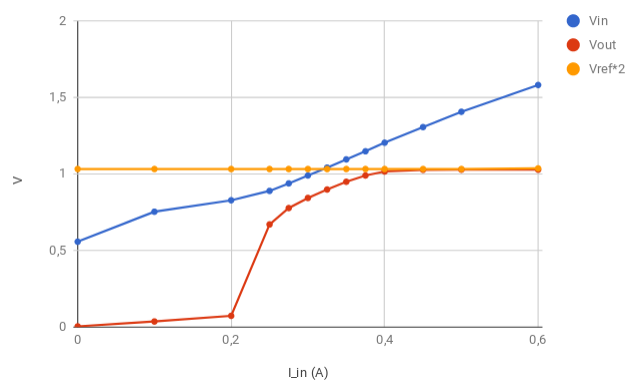
\includegraphics[scale=.5]{Immagini/provaSLDO5}
\caption{.}
\label{provaSLDO5}
\end{figure}

Le prime curve di IV sono state eseguite sullo shunt da 0.5 A in cui era possibile regolare solo $V_{ref}$, di seguito è riporto il grafico ottenuto andando a variare la corrente in ingresso in configurazione senza carico applicato al $V_{out}$,figura \ref{provaSLDO5}. Questa è quindi una situazione in cui tutta la corrente fornita dall'alimentazione viene assorbita dallo shunt,  prendendo l'andamento asintotico e disinteressandoci della parte iniziale del grafico, che corrisponde al power up dello ShuntLDO, riportiamo in tabella alcuni valori di interesse: 

\[
\begin{array}{ccccc}

\toprule
V_{ref} & V_{out} & 2 \cdot V_{ref}- V_{out} & R_{eff} & V_{offset} \\

\midrule

0.516 V & 1.028 V & 8 mV & 2.0 \Omega & 0.40 V \\

\bottomrule
\end{array}
\]
In questa prima misura non era applicato nessun carico al $V_out$, dunque tutta la corrente in ingresso scorre nello Shunt, questa misura ci aiuterà in un confronto successivo con situazioni in cui è presente un carico sia statico che dinamico. 

Un'altra misura di test, che è stata eseguita con questo prototipo di shunt prima del passaggio alla versione da 2A, è un serie di due shunt entrambi con un carico resistivo di 4 $\Omega$. I due ShuntLDO hanno $V_{ref}$ diversi $V_{ref1}=0.497$ V e $V_{ref2}=0.553$ V. Inoltre è possibile separare l'alimentazione del bandgap, presente sulla PCB, da quella dello SLDO. Il compito del bandgap è generare una tensione di riferimento regolabile con un potenziomentro e utilizzata dallo ShuntLDO come $V_{ref}$.
Possiamo vedere a confronto il diverso comportamento nel caso in cui VCC, tensione che alimenta il bandgap sia esterna, con il caso in cui la tensione VCC sia cortocircuitata con l'ingresso di $I_{in}$ e dunque si trovi a tensione uguale a $V_{in}$, figura \ref{SLDO5Serie}. In questo confronto va tenuto conto che il bandgap ha un regimen di lavoro compreso tra  i 2 e i 18 V. 
\begin{figure}
\centering
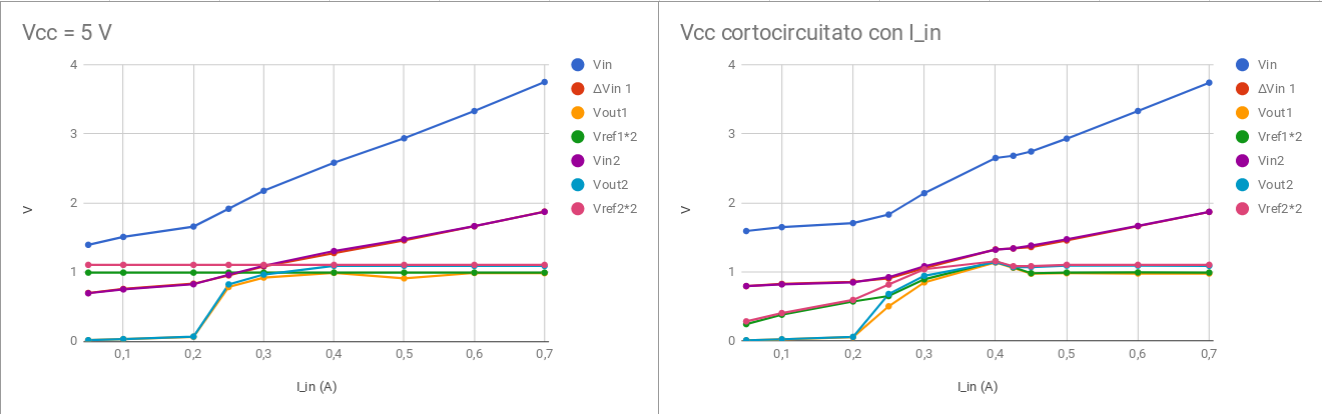
\includegraphics[scale=.3]{Immagini/SLDO5Serie}
\caption{A sinistra i bandgap sono alimentati esternamente, a destra sono alimentati tramite $V_{in}$.}
\label{SLDO5Serie}
\end{figure}
Quello che si può notare dai grafici è che fintanto che la tensione di ingresso non supera circa 1 V il bandgap non riesce a generare il giusto livello di tensione $V_{ref}$ e ciò ha come conseguenza un $V_{out}$ non stabile, ovvero si arriva ad una stabilità del $V_{out}$ a correnti più elevate.

\begin{figure}
\centering
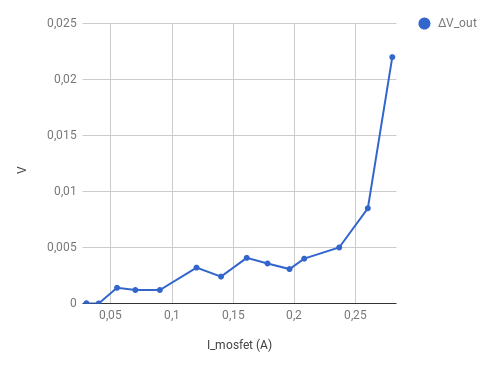
\includegraphics[scale=.4]{Immagini/SLDO5singlepulse}
\caption{Entità degli undershoot in tensione in funzione della corrente assorbita dal mosfet.}
\label{SLDO5singlepulse}
\end{figure}

Una prima misura di test può essere fatta anche in configurazione di carico dinamico, per poi riproporla in modo più approfondito ed esaustivo nelle sezioni successive utilizzando però il prototipo da 2A.
Nella PCB di test è presente in parallelo all'uscita di $V_{out}$ un in serie ad una resistenza, il cui comportamento può essere controllato esternamente applicando una tensione al gate. 
La corrente assorbita dal mosfet, può essere ricavata andando a misurare la caduta di tensione sulla resistenza. La prima misura di interesse è vedere quanto il $V_{out}$ sia sensibile a variazioni veloci di carico. In figura \ref{SLDO5singlepulse} è riportato l'andamento dell'undershoot in funzione della corrente assorbita dal mosfet. Va tenuto presente che le misure sono state effettuate con una alimentazione in corrente $I_{in} = 0.5$, un $V_{ref} \sim 0.5$ V e un carico resistivo su $V_{out}$ di 4 $\Omega$. Questo perchè nel momento in cui il carico dinamico più il carico statico assorbono insieme una corrente maggiore di quella totale in ingresso il sistema va in crisi. Gli effetti visibili quando $I_{mosfet} + I_{load} > I_{in}$ non hanno quindi direttamente a che vedere con il comportamento dello SLDO. Si può vedere dal grafico \ref{SLDO5singlepulse} come gli undershoot rimangano inferiori a 10 mV fin tanto che $I_{mosfet}$ rimane sotto gli 0.250 A, valore oltre cui $I_{mosfet} + I_{load} > I_{in}$\footnote{$I_{load}$ è la corrente che scorre nel carico resistivo, in questo caso $I_{load} = \dfrac{V_{out}}{R} = 0.250$A}. 

Lo stesso test può essere eseguito mettendo due SLDO in serie ed andando a variare dinamicamente il carico di uno dei due, verificando se esternamente queste variazioni siano visibili, e quindi se influenzino l'altro elemento della catena seriale. 
Dal momento che l'interesse maggiore è per il prototipo a 2 A questo tipo di misura non è stato riportato nel caso dello SLDO da 0.5A, in quanto lo scopo di questa prima parte è quello di introdurre un certo tipo di approcci e per prendere confidenza con gli argomenti trattati.

\section{ShuntLDO 2A}
%\begin{figure}
%\centering
%\includegraphics[scale=.3]{Immagini/PCB2A}
%\caption{.}
%\label{PCB2A}
%\end{figure}

\section{Comportamento statico}
Rispetto a quanto visto in precedenza, nella versione da 2 A è possibile gestire anche l'offset attraverso un potenzionetro RP2 che va ad agire sulla tensione in uscita generata dal bangap, la stessa che viene utilizzata per generare $V_{ref}$ regolando un secondo potenziometro RP1. La parte di caratterizzatione statica è di nuovo eseguita andando a variare la corrente di alimentazione in ingresso e al contempo misurando $V_{out}$, $V_{ref}$ e $V_{in}$, figura \ref{SLDO2Astatic}.

\begin{figure}
\centering
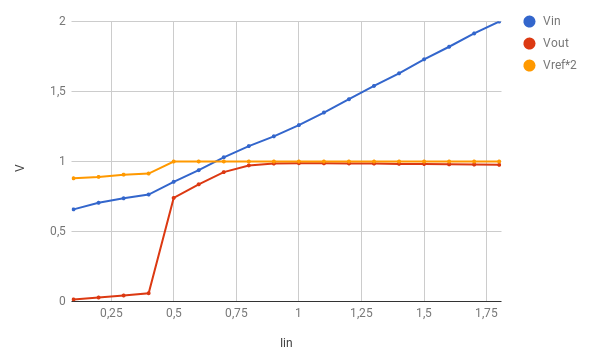
\includegraphics[scale=.5]{Immagini/SLDO2Astatic}
\caption{.}
\label{SLDO2Astatic}
\end{figure}

Questo andamento è stato ottenuto ponendo\footnote{Per selezionare il valore voluto è necessario regolare il potenziometro RP1 che si trova in serie al bandgap sulla PBC.} $V_{ref} = 0.5$ V e applicando un carico resistivo di 1 $\Omega$ a $V_{out}$. Il bandgap è alimentato esternamente con una tensione di 5 V. 
Come si vede dal grafico \ref{SLDO2Astatic} delle IV Vref non è costante nella parte iniziale, questo può essere dovuto al fatto che nella fase in cui lo shunt LDO non è attivo, si ha uno scorrimento di corrente nel ramo di $V_{ref}$. Dato che in serie al bandgap c'è il potenziometro, se si ha una corrente che scorre si viene a creare una caduta di tensione. Questa caduta di tensione fa si che il $V_{ref}$ inizialmente sia più basso. Idealmente nel ramo di $V_{ref}$ dovrebbe scorrere una corrente molto piccola in regime di lavoro\footnote{Questo perchè nello SLDO il $V_{ref}$ è in ingresso al comparatore A1 \ref{SLDO2A} e viene confrontato con una tensione che sarà circa uguale in una situazione di equilibrio. La corrente che scorre dunque tra ingresso + e - sarà piccola, anche perchè il comparatore in ingresso ha ua grossa resistenza.}, mentre al momento dell'accensione, all'ingresso di A1 si ha una notevole differenza tra + e -, e quindi scorrerà una corrente maggiore, questo è causa di una variazione del $V_ref$. Di seguito riportiamo in tabella alcuni valori di interesse: 

\[
\begin{array}{ccccc}

\toprule
V_{ref} & V_{out} & 2 \cdot V_{ref}- V_{out} & R_{eff} & V_{offset} \\

\midrule

0.500 V & 0.980 V & 20 mV & 0.880 \Omega & 0.40 V \\

\bottomrule
\end{array}
\]

\subsection{Differenze tra GND PCB e GND SLDO}
Prima del passaggio alla caratterizzazione statica è interessante fare alcune riflessioni per porre attenzione su un aspetto che influenza le misure. 
Tutte le tensioni misurate, come per esempio il $V_{out}$, sono eseguite utilizzando pin sulla PCB. Questo vuol dire che per esempio quando viene misurato $V_{out}$ quello che viene letto sull'oscilloscopio o attraverso i multimetri è la differenza di tensione tra il pin di $V_{out}$ sulla PCB e la terra (GND) della medesima. Dal momento che questi punti di misura sono collegati al $V_{out}$ dello $\mathrm{ShuntLDO}$ attraverso wire bond si ha una certa resistenza che a sua volta genera una caduta di tensione. Questa caduta di tensione dipende dalla corrente assorbita dal carico, dunque nel caso di una caratterizzazione con carico fisso si presenta come un offset, mentre nel caso il carico sia dinamico varia al variare della corrente. 
Il valore di questa resistenza dipende dal numero di wire bond eseguiti, questi wire bond si presentano con tante resistenze in parallelo. Dunque maggiore sarà il numero di questi ultimi minore sarà il valore della resistenza equivalente e dunque minore sarà l'effetto su $V_{out}$. Questo problema è riportato schematicamente in figura \ref{Ground}.

\begin{figure}
\centering
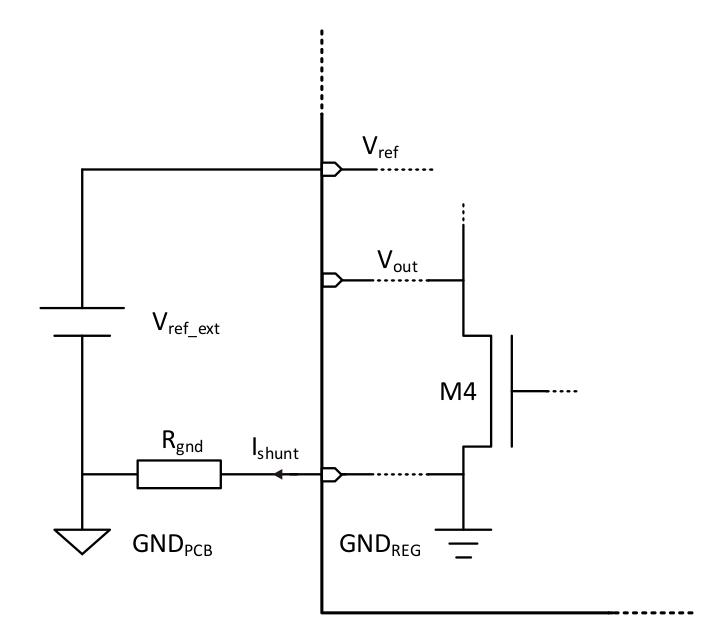
\includegraphics[scale=.3]{Immagini/Ground}
\caption{Differenze tra $\mathrm{GND_{PCB}}$ e $\mathrm{GND_{REG}}$ nella configurazione ShuntLDO, causate dalla corrente di shunt.}
\label{SLDO2Astatic}
\end{figure}

Recapitolando, nella configurazione di ShuntLDO una frazione della corrente in ingresso scorre attraverso il transistor di shunt (M4), questa corrente scorre nella linea di terra del regolatore $\mathrm{GND_{REG}}$ e da qui, attraverso i wire bond è collegata alla terra della PCB ($\mathrm{GND_{PCB}}$). La resistenza di questa linea, schematizzata in figura con una resistenza $\mathrm{R_{GND}}$, è la causa della differenza in tensione tra la terra della PCB e dello Shunt. Questo spiega anche il fatto che $V_{ref_ext}$ sia leggermente maggiore di $V_{out}$. Infatti  $V_{ref_ext}$ è esterno allo shunt e dunque l'effettiva tensione di riferimento vista dallo shunt è minore. Il $V_{out}$ realmente prodotto dallo ShuntLDO sarà:
\begin{equation}
V_{out} = 2 \cdot V_{ref} = 2 \cdot ( V_{ref {\_} ext} - I_{shunt} \cdot R_{gnd} )
\end{equation}

Questo effetto è appena visibile in figura \ref{SLDO2Astatic}, dove all'aumentare della corrente $V_{out}$ si ha una lieve flessione della tensione in uscita. Facendo un fit lineare dei punti si ottiene una pendenza di - 0.015 $\Omega$. 
La pendenza ottenuta del fit non è unicamente data dai wire bond ma ha un cotributo aggiuntivo dato dalla resistenza delle piste e dei connettori. 
Una misura più precisa può essere eseguita sfruttando i pin $\mathrm{V_{out{\_}Sense}}$ e $\mathrm{I_{out {\_} Sense}}$, rispettivamente indicati sulla PCB con P5 e P6. 
Questi due pin di monitoraggio sono collegati rispettivamente al $V_{out}$ del regolatore e al GND sempre del regolatore. 
Essendo piste in cui non scorre corrente, l'effetto resistivo di wire bond e piste è eliminato ed è possibile misurare il il valore di tensione del GND locale.

\begin{figure}
\centering
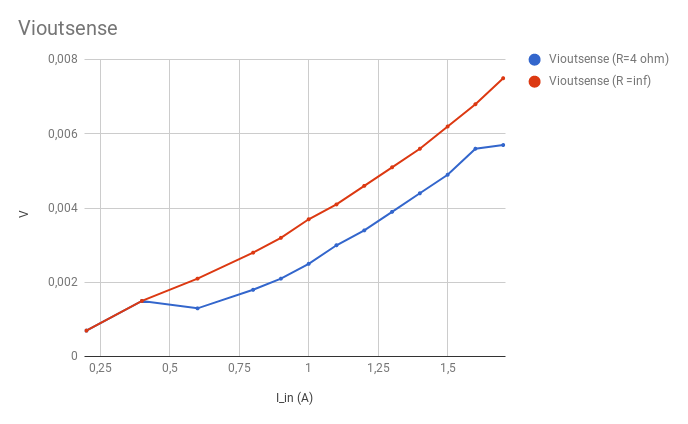
\includegraphics[scale=.4]{Immagini/Viout}
\caption{Andamento della tensione del GND dello shunt rispetto al GND della PCB al variare della corrente di alimentazione del circuito.}
\label{VioutSense}
\end{figure}

Si è proceduto a misurare il valore di tensione sul pin $I_{out{\_}Sense}$ al variare della corrente di alimentazione $I_{in}$. 
La misura è stata eseguita per due diversi valori di carico statico $4$ $\Omega$ e $\inf$, con il valore infinito si intende la configurazione in cui il carico è assente e dunque il circuito tra $V_{out}$ e GND è aperto. 
In figura \ref{VioutSense} è possibile vedere come le due diverse configurazioni di carico influenzino la misura con un offset. 
Infatti nei due casi la pendenza è la stessa e dà un'indicazione del valore resistivo dei wire bond, l'offset invece rispecchia il fatto che lo shift di tensione è dato dalla corrente che scorre verso il GND del chip, che nel caso in cui il carico richieda più corrente diminuisce. Ad esempio a 1 A con i carico resistivo da 4 $\Omega$ la corrente che effettivamente scorre verso GND nello shunt è 0.75 A (questo nel caso $V_{out} = 1 V$).

\[
\begin{array}{cccc}

\toprule
Slope red & Slope blue & offset red & offset blue \\

\midrule

4 m \Omega & 4 m\Omega & -1 mV  & -2 mV \\

\bottomrule
\end{array}
\]

Il valore di questa resistenza è molto piccolo e come detto dipende in prima approssimazione dal numero di wire bond. Fintanto che lo ShuntLDO è utilizzato come circuito a se stante su una PCB di test questo aspetto risulta secondario, in quanto non ci sono problemi di spazio e si può utilizzare un gran numero di connessioni per ridurre al minimo differenze tra $\mathrm{GND_{PCB}}$ e $\mathrm{GND_{REG}}$.   

  
\subsection{Offset}
Come detto in precedenza nella versione da 2 A è possibile regolare esternamente il $V_{offset}$. 
Una tensione di offset alta consente di raggiungere il punto di lavoro prima, cioè con un minor consumo di corrente, mentre un valore di $V_{offset}$ basso ha l'effetto contrario. Questo effetto lo si può verificare andando a misurare la tensione di output $V_{out}$
\begin{figure}
\centering
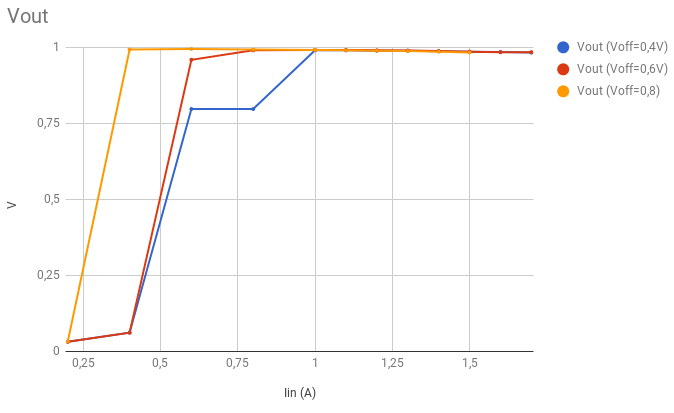
\includegraphics[scale=.4]{Immagini/VoutVsVoffset}
\caption{VoutVsVoffset.}
\label{VoutVsVoffset}
\end{figure}

\begin{figure}
\centering
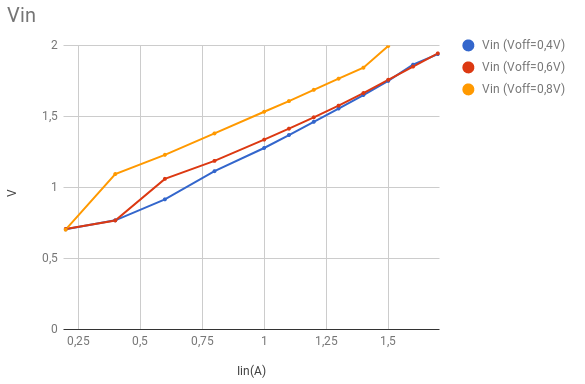
\includegraphics[scale=.4]{Immagini/VinVsVoffset}
\caption{VinVsVoffset.}
\label{VinVsVoffset}
\end{figure}
\[
\begin{array}{ccc}

\toprule
Offset 0.4 V & Offset 0.6 V & Offset 0.8 V  \\

\midrule

0.352 V & 0.539 V & 0.756 V \\

\bottomrule
\end{array}
\]

\section{Comportamento dinamico}

\begin{figure}
\centering
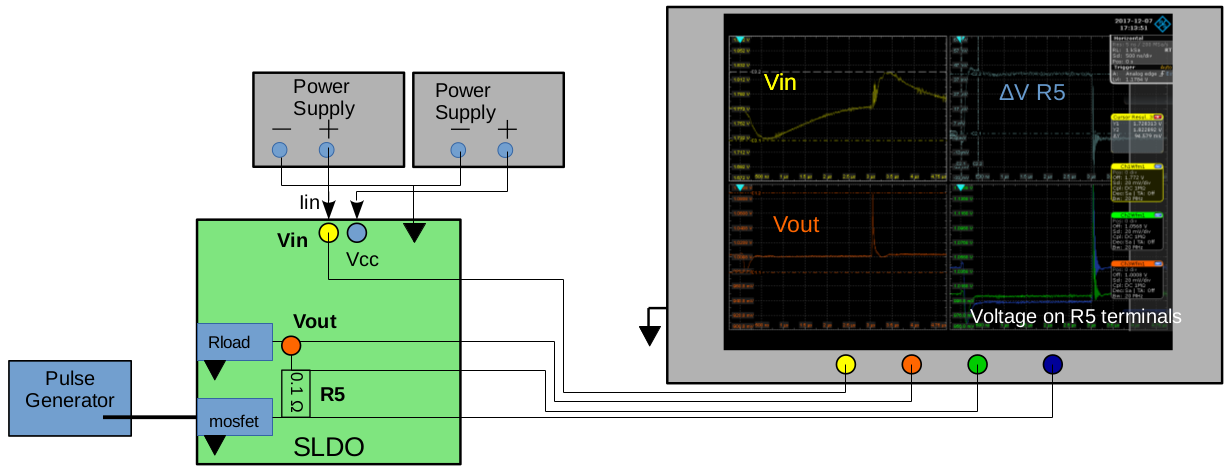
\includegraphics[scale=.3]{Immagini/SetupScheme}
\caption{Schema del setup per lo studio del comportamento dinamico dello SLDO.}
\label{Setupscheme}
\end{figure}

Oltre alla caratterizzazione statica è interessante studiare il comportamento dello SLDO in risposta ad una variazione dinamica del carico, andando a focalizzare l'attenzione sulla velocità dello shunt nel riequilibrare il consumo in corrente. La risposta dinamica è dipendente da fattori quali il punto di lavoro a cui si trova lo SLDO, il tempo in cui avviene la variazione di carico e l'entità di tale variazione.
Il setup di queste misure è rappresentato schematicamente in figura \ref{Setupscheme}. Il circuito è alimentato tramite un generatore di corrente a $1.5A$ (CONTROLLARE) e $Vref=0.5 $, dunque ci aspettiamo una tensione all'uscita di $1V$. Al fine di introdurre un carico dinamico, in parallelo al carico statico, è presente un mosfet in serie ad una resistenza R5 di $0.1 \Omega$.
La corrente assorbita dal mosfet, indicata con $I_{mosfet}$ sarà perciò ricavata misurando la caduta di tensione sulla resistenza. Il mosfet è pilotato tramite un generatore di impulsi, a seconda dell'ampiezza del segnale inviato il gate del mosfet viene più o meno aperto, permettendo il passaggio maggiore o minore di corrente.
per quanto riguarda la durata dell'impulso si è scelto di tenere fronte di salita e discesa separati in modo da osservare separatamente gli effetti dovuti al fronte di salita da quelli di discesa. 
Le variazioni di carico dovute al chip in confronto possono essere di minor durata, lo scopo di queste misure è però vedere gli effetti che si hanno al passaggio da un certo consumo di corrente ad uno maggiore e viceversa, un impulso di breve durata avrebbe il problema di sovrapporre questi due effetti, non permettendo di valutarne l'effettiva entità, in quanto i contributi sono opposti e su tempi si sovrappongono cancellandosi.
In queste misure l'attenzione sarà focalizzata su variazioni di $V_{in}$ e $V_{out}$ in ampiezza e sul tempo di recupero al variare di $I_{mosfet}$ per una data $R_{load}$.

L'introduzione di questo carico parallelo alla resistenza connessa a $V_{out}$ tramite il molex J1 è possibile andando a cortocircuitare con un jumper i pin P10 sulla PCB. Come si può notare già dalle prime misure con l'oscilloscopio l'utilizzo del mosfet come carico dinamico non è esente da problematiche che vanno ad alterare i segnali, compromettendone una corretta interpretazione.
 Prendendo a riferimento la figura \ref{TransientTest} si nota innanzitutto un'asimmetria nelle variazioni di $V_{out}$, posto in basso a sinistra e di colore arancione, mentre in $V_{in}$, posto in alto a sinistra e di colore giallo, la risposta è simmetrica. In azzurro è riportata la differenza tra le tensioni misurate ai capi di R5, riportate in blu e in verde, da cui è possibile calcolare la corrente che scorre tra Drain e Source del mosfet. 
Sono visibili delle oscillazioni in corrispondenza del momento in cui il mosfet si spegne e smette di assorbire corrente. Questo comportamento si riflette su $V_{out}$, ed è quindi all'origine dell'asimmetria. Questo aspetto è stato approfondito prima di procedere a misure della risposta dinamica nelle varie combinazioni $I_{mosfet}$-$R_{load}$, al fine di capire a cosa fosse dovuto, sospettando un contributo del mosfet non trascurabile.
In questa prima fase l'impulso utilizzato ha le seguenti caratteristiche: frequenza $50 Hz$, durata $3 \mu s$, durata del fronte di salita $40 ns$.
\begin{figure}
\centering
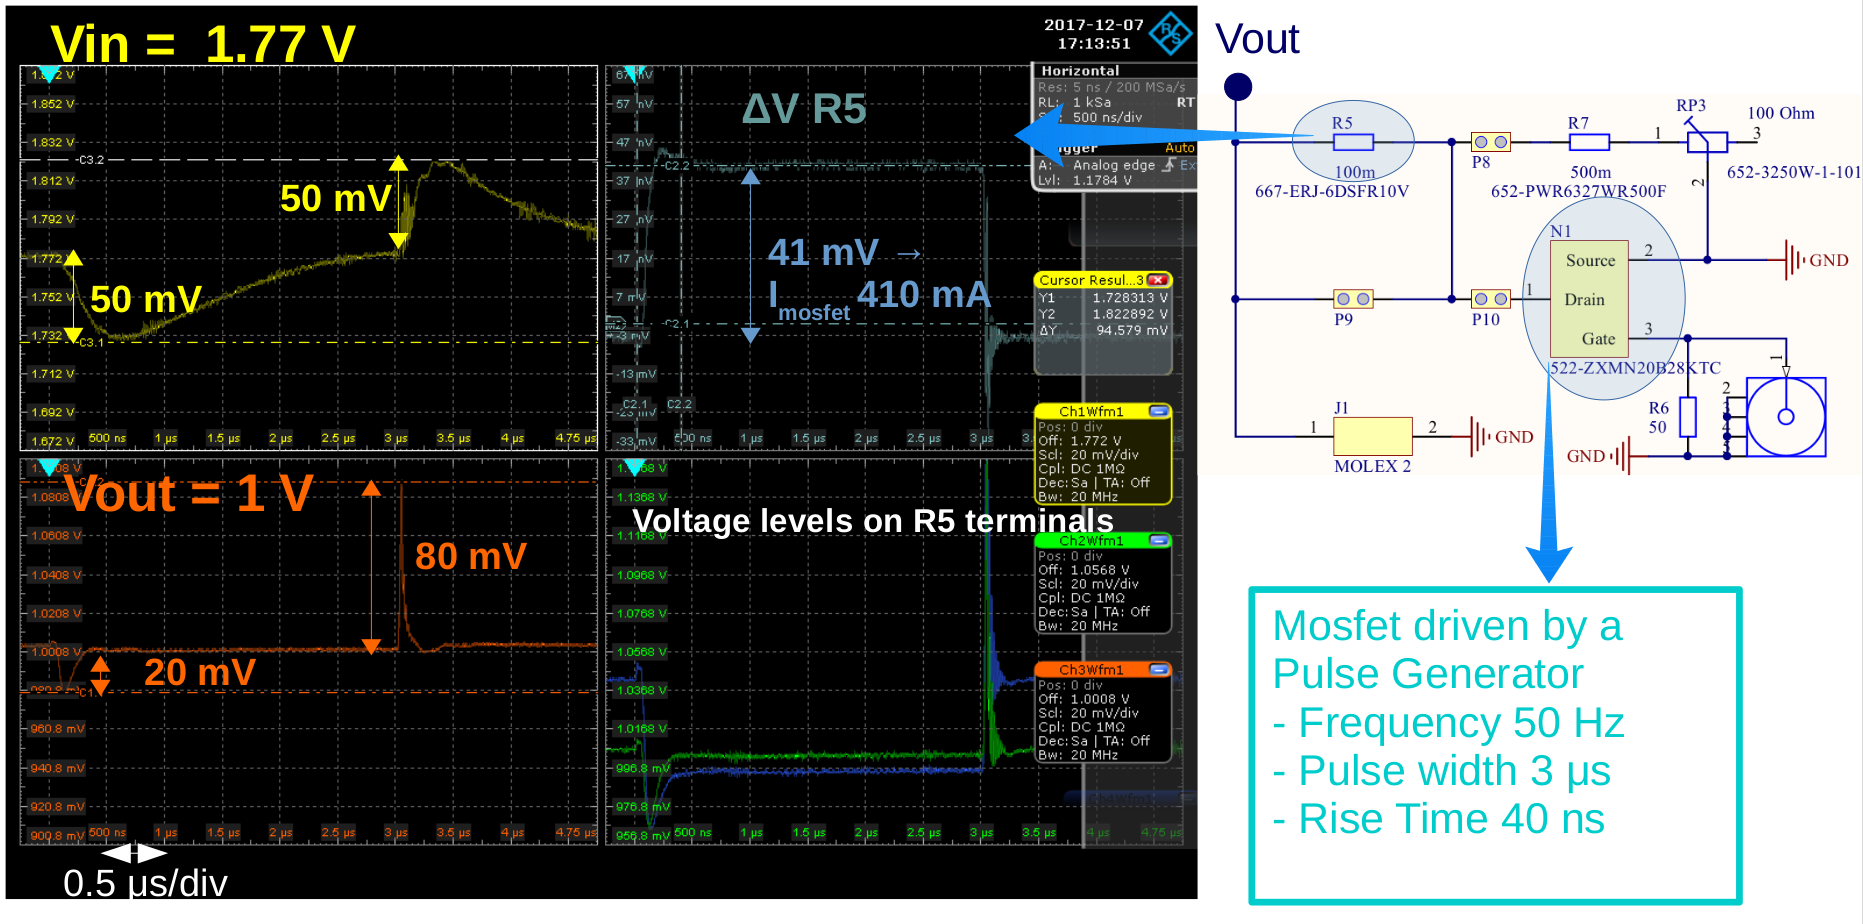
\includegraphics[scale=.2]{Immagini/TransientTest}
\caption{.}
\label{TransientTest}
\end{figure}

Per esaminare il comportamento del mosfet in risposta all'impulso mandato sul gate si è proceduto ad isolare questa parte del circuito dal resto della PCB andando a connettere sul pin P10 connesso al drain una resistenza in serie ad una batteria (la batteria ricopre il ruolo di $V_{out}$, mentre la resistenza è necessaria alla misura delle correnti che scorrono da batteria a drain. La resistenza utilizzata è $R=2.7 \Omega$ e misurandone la caduta di tensione è possibile calcolare la corrente.

\begin{figure}
\centering
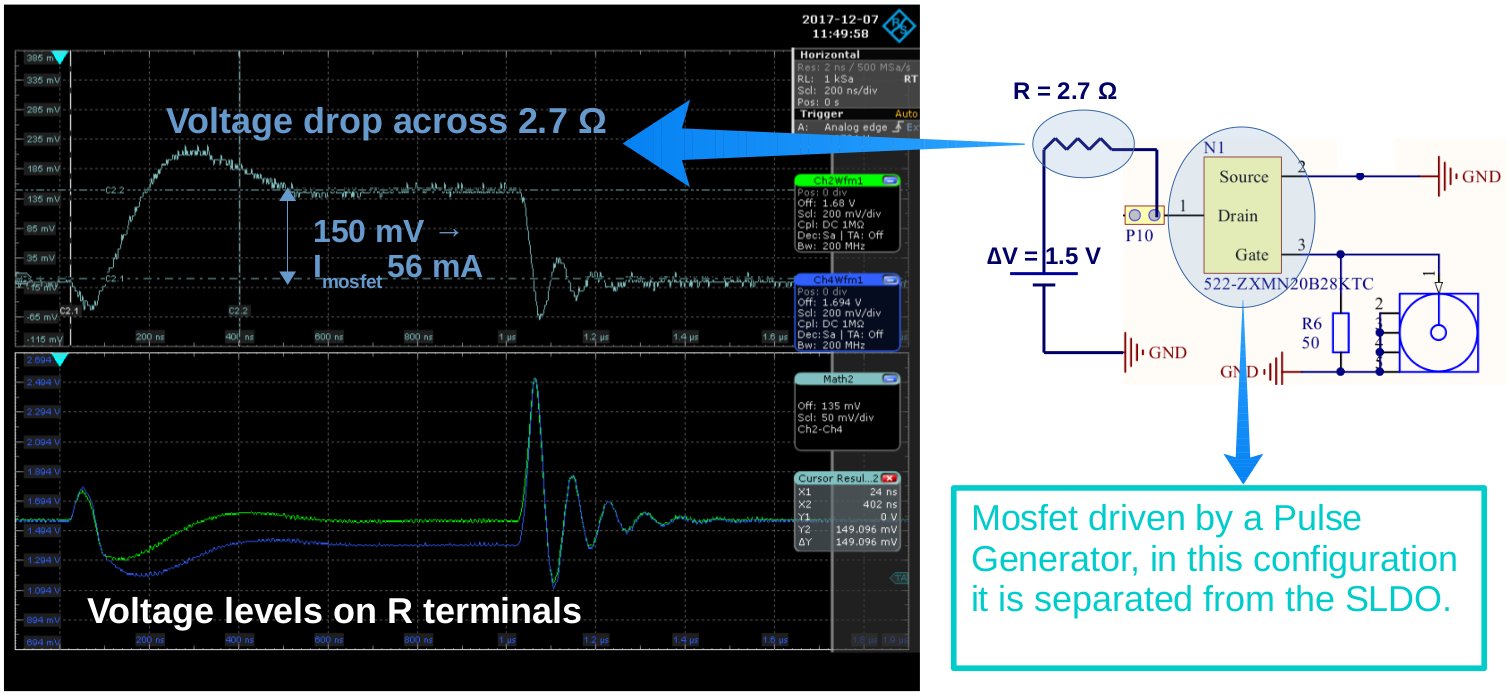
\includegraphics[scale=.3]{Immagini/MosfetBehaviour}
\caption{.}
\label{MosfetBehaviour}
\end{figure}

Come è possibile vedere dalla figura \ref{MosfetBehaviour}, le oscillazioni sono presenti anche una volta isolato il mosfet, segno che sono generate da quest'ultimo nel momento in cui il canale che collega drain e source si interrompe, inoltre il fronte di salita è circa 100 ns e non 40 ns come ci aspetteremmo da un mosfet ideale con risposta istantanea. Andando a esaminare la documentazione del mosfet presente sulla PCB (ZXMN20B28KTC http://www.mouser.com/ds/2/115/ZXMN20B28K-94822.pdf) si può verificare che effettivamente il tempo di accensione è superiore a 40 ns (Turn-on rise time 76,9 ns) e inoltre sono presenti capacità in ingresso di $358 pF$. Tutto questo rende impossibile vedere la risposta dello SLDO a segnali più veloci della risposta del mosfet, motivo per cui le misure successive sono state prese impostando un tempo di salita del segnale del generatore di impulsi di $200 ns$.
In figura \ref{RiseTime} è visibile come la situazione precedente, in cui l'impulso ha un tempo di salita di 40 ns, migliora visibilmente passando a 200 ns.
\begin{figure}
\centering
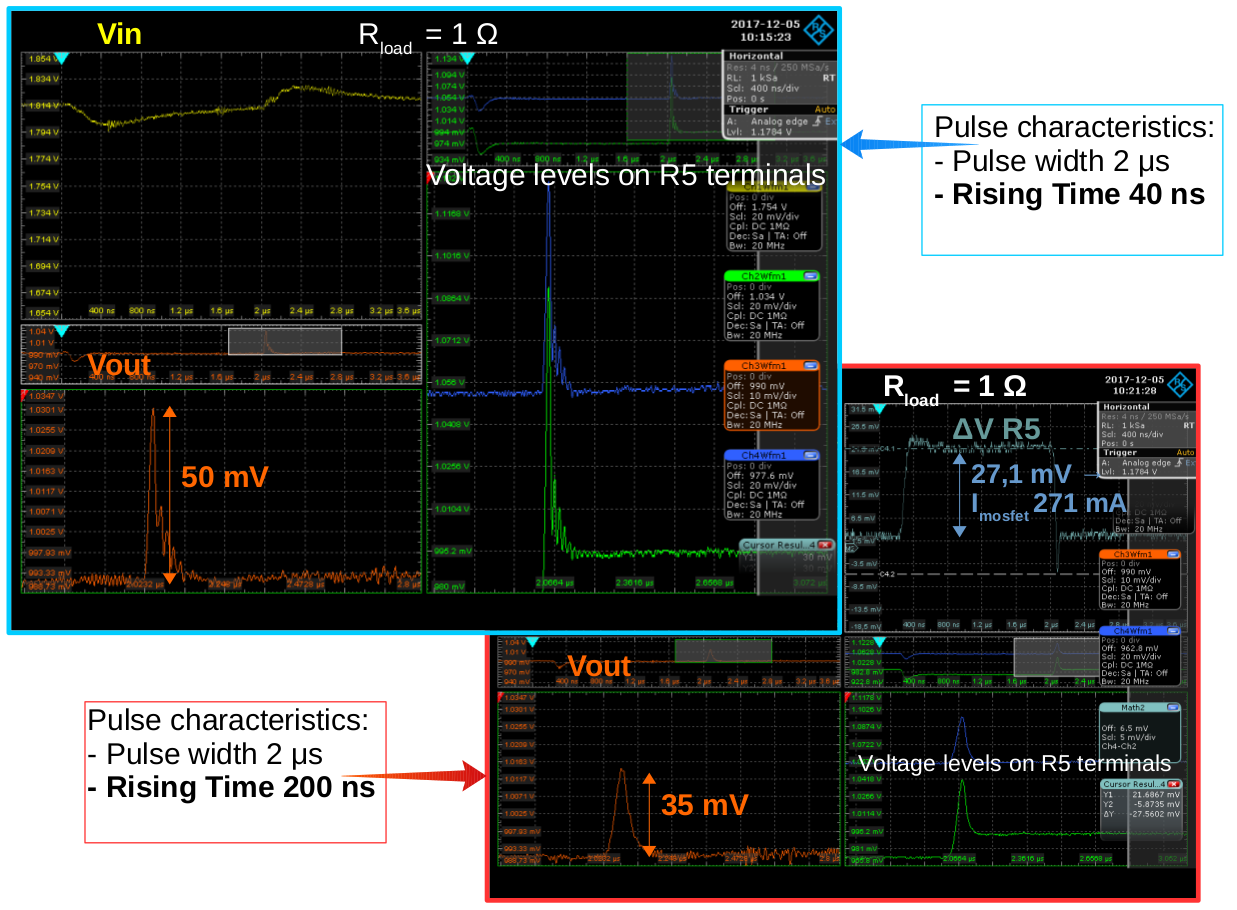
\includegraphics[scale=.3]{Immagini/RiseTime}
\caption{.}
\label{RiseTime}
\end{figure}
A questo punto si è proceduto con le misure di $V_{in}$ e $V_{out}$ per tre differenti valori di $R_{load}$ al variare di $I_{mosfet}$. I valori di $R_load$ scelti sono stati $1 \Omega$, $2.1 \Omega$ e $4 \Omega$, che dato $V_{out}=1V$ corrispondono rispettivamente a correnti  $I_{load}$ di $1A$, $0.475 A$ e $0.250A$. A questo punto per vari valori di $I_{mosfet}$ sono stati misurate le variazioni in ampiezza e il tempo di recupero di $V_{in}$ e $V_{out}$.

Il primo punto da notare è il differente tempo di recupero tra $V_{in}$ e $V_{out}$, molto più lungo dell'ordine dei $\mu s$ e dipendente dall'entità di $I_{mosfet}$ per il primo mentre per il secondo ha durata di circa $300 ns$ indipendentemente dal valore di $I_{mosfet}$.
Va ricordato che lo SLDO è alimentato in corrente con $1.5A$, dunque nel momento in cui $I_{load}+I_{mosfet}$ raggiungono valori vicini o addirittura superiori  a $I_{in}$ si ha un crollo della tensione in ingresso e del $V_{out}$. Questo è un effetto aspettato in quanto si sta chiedendo allo SLDO di fornire una corrente superiore a quella a sua disposizione.


Per ciascun valore di $R_{load}$, come detto in precedenza, è stata fatta variare la corrente assorbita dal mosfet $I_{mosfet}$ ed è stato misurato l'effetto di undershoot e overshoot sulle tensioni di $V_{out}$ e $V_{in}$.
 

